% z4.tex

\documentclass[tikz]{standalone}

\begin{document}
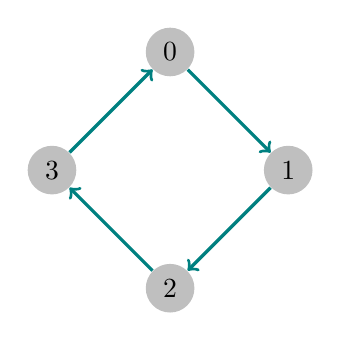
\begin{tikzpicture}[ele/.style = {circle, minimum size = 6pt, fill = lightgray}]
  \foreach \i [count = \j from 0] in {90, 0, -90, -180} {
	\node (\j) [ele] at (\i:1.5) {$\j$};
  }

  \foreach \i in {0, 1, 2} {
	\def\next{\the\numexpr\i+1}
	\draw[->, teal, very thick] (\i) to (\next);
  }
  \draw[->, teal, very thick] (3) to (0);
\end{tikzpicture}
\end{document}
